\chapter{Project schedule}\label{ch:schedule}
    \section{Gantt Chart}

    We built a Gantt Chart for the project schedule to allow us to keep track of the time. We couldn't create tasks that would indicate a slippage since it would disrupt the critical path. As a result, we increased the time alloted to each assignment, reflecting the slippage. We included slippage due of other university homework, exams and even illness.

    As shown in Figure \ref{fig:gantt_chart}, teh highlighted tasks illustrate the project's critical path. We devided the project into three Sprints because we are utilizing the scrum methodlogy. The first Sprint consists only of require collection and project planning. The second Sprint includes the sprint plan, as well as the software and hadrware designs and implementations. The third Sprint contains the sprint plan as well as the system's final implementation, in which the walking aid will connect with our system, the wrist device. The final task of each Sprint is a milestone, signaling the Sprint's completion.

    \begin{figure}[H]
      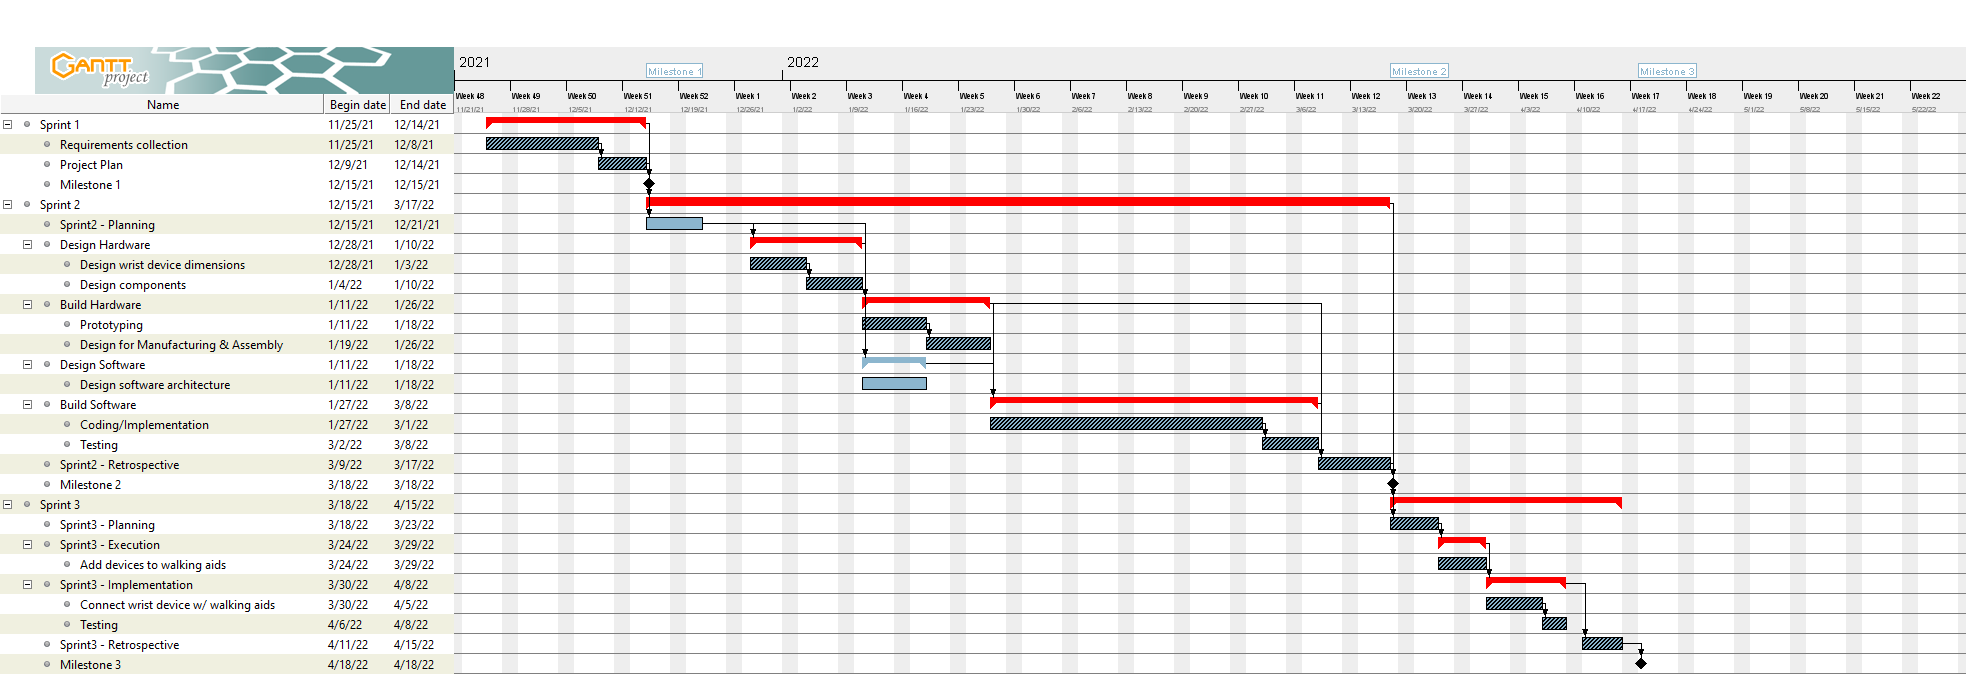
\includegraphics[width=\linewidth]{graphics/Gantt_Chart.png}
      \caption{Gantt Chart}
      \label{fig:gantt_chart}
    \end{figure}

    \section{Activity Network Diagram}

    In terms of scheduling, an activity diagram is just a significant as designing a Gantt Chart. We merged several of the jobs that were introduced to Gantt Chart into one task to make the activity network diagram more undestandable. However, this has no bearing on the total time requried to finish the project. According to Figure \ref{fig:activity_network_diagram}, the total time requried is 107 working days.

    \begin{figure}[H]
      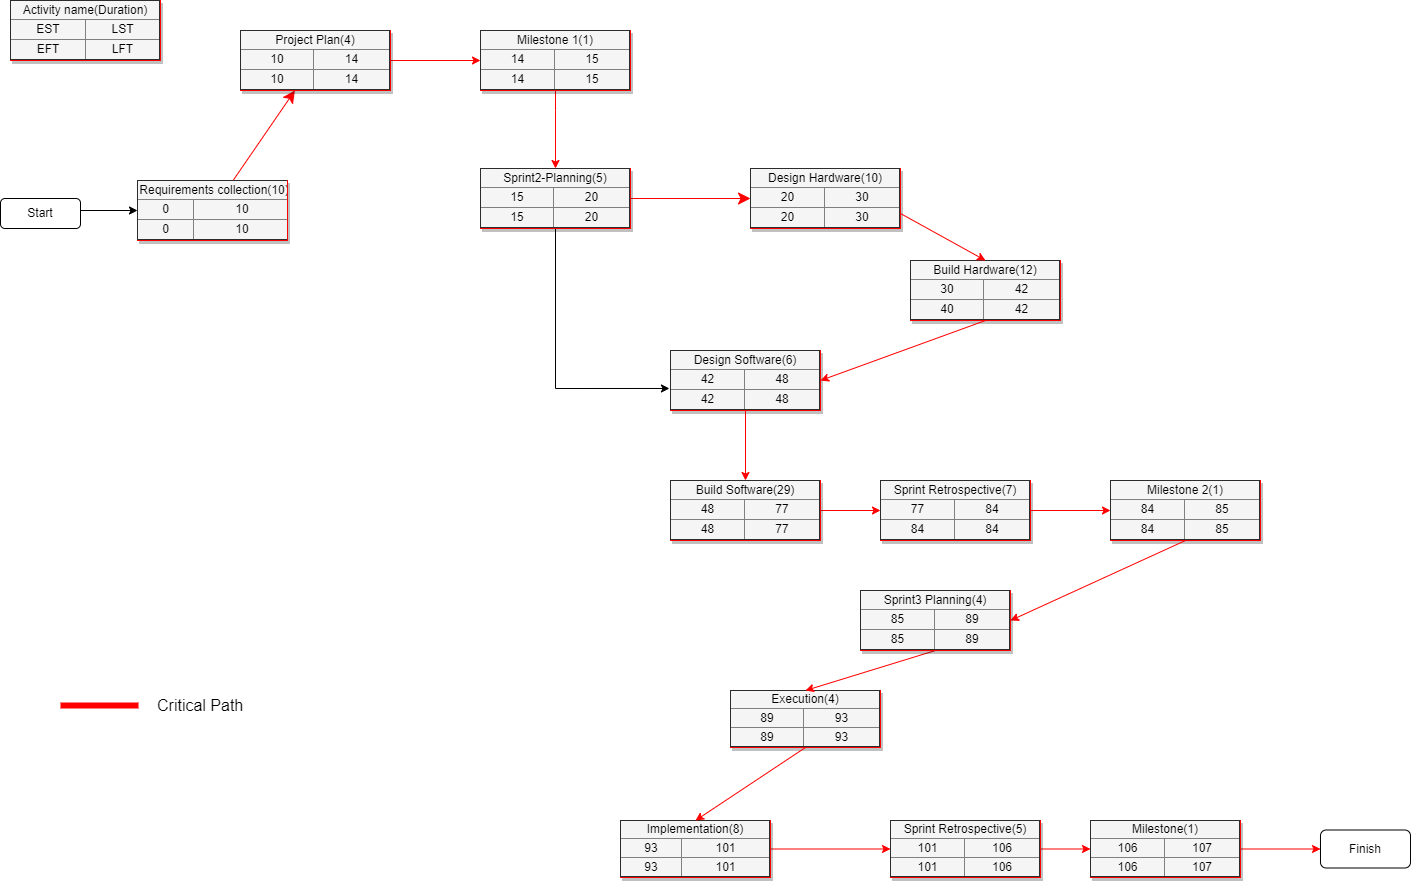
\includegraphics[width=\linewidth]{graphics/AND.drawio.png}
      \caption{Activity Network Diagram}
      \label{fig:activity_network_diagram}
    \end{figure}
